% @file  Exact Template Attacks with spectral computation.tex
% sa     https://www.asianhost.org/2024/
% sa     https://www.overleaf.com/project/6672f0010eb5156602f39982

% Important Dates
%  - Paper submission: July 14, 2024, 23:59:59 JST
%  - Acceptance: September 11, 2024
%  - Camera-ready version: October 30, 2024
%  - On-site conference: December 16-18, 2024

% ePrint deadline:
% If you wish to revise or withdraw your submission, you should visit
% https://eprint.iacr.org/revise?name=xxxx/103744&confirmation=BLcdgma and enter the following information:
%   Paper ID: xxxx/103744
%   Confirmation: BLcdgma


%\documentclass[conference,onecolumn]{IEEEtran}
\documentclass[conference,twocolumn]{IEEEtran}
\IEEEoverridecommandlockouts
% The preceding line is only needed to identify funding in the first footnote. If that is unneeded, please comment it out.
\usepackage{cite}
\usepackage{amsmath,amssymb,amsfonts}
\usepackage{algorithmic}
\usepackage{graphicx} %\pdfminorversion=7 % pour l'import des fichiers *.pdf externes
\usepackage{textcomp}
\usepackage{xcolor}
\def\BibTeX{{\rm B\kern-.05em{\sc i\kern-.025em b}\kern-.08em
    T\kern-.1667em\lower.7ex\hbox{E}\kern-.125emX}}


\setlength {\marginparwidth }{2cm} 
\usepackage{todonotes}

%%%%%%%%%%%%%%%%%%%%%%%%%%%%%%%%%%%%%%%%%%%%%%%%%%%%%%%%%%%%%%%%%%%%%%
\usepackage{mathtools}
\usepackage{wrapfig}
\usepackage{color}
\usepackage{url, rotating}
%\usepackage{boxedminipage}
\usepackage{multirow}
%\usepackage[table,xcdraw]{xcolor}
\usepackage{newlfont}
\usepackage{float}
%\usepackage{epsfig,titling,array}
%\usepackage{algpseudocode, algorithm, algorithmicx}
%%%%%%%%%%%%%%%%%%%%%%%%%%%%%%%%%%%%%%%%%%%%%%%%%%%
%%%%%%%%%%%%%%%%%%%%%%%%%%%%%%%%%%%%%
% Load basic packages
%\usepackage{balance}  % to better equalize the last page
%\usepackage{flushend} % Balancing columns at last page
% See section XIII of https://ras.papercept.net/conferences/support/files/IEEEtran_HOWTO.pdf
\usepackage{times}    % comment if you want LaTeX's default font
\usepackage{soul}
%\usepackage{subfig}
%\usepackage[caption=false]{subfig}
%%%%%%%%%%%%%%%%%%%%%%%%%%%%%%%%%%%%%%%%%%%%%%%%%%%%
\usepackage{subfigure}
%\usepackage{pdfpages}
%\usepackage{caption}
%.........................
%\usepackage{subcaption}
%%%%%%%%%%%%%%%%%%%%%%%%%%%%%%%%%%%%%%%%%%%%%%%%%%%

\usepackage{booktabs}
\usepackage{listings}
\usepackage{fancyhdr}
\usepackage{afterpage}
\usepackage{svg}
\usepackage{longtable}
\usepackage{amsmath,amsfonts,amssymb}
%\usepackage{chemist}
%\usepackage[version=4]{mhchem}
%\usepackage{ gensymb }
\usepackage[boxed,vlined,linesnumbered]{algorithm2e} 
% Unused options: noend
\usepackage{hyperref}%.......................
%\usepackage[colorlinks]{hyperref}
\usepackage{tikz}
%%%%%%%%%%%%%%%%%%%%%%%%%%%%%%%%%%%%%%%%%%%%%%%%%%%

%\usepackage[french,english]{babel}
\usepackage[english]{babel}
%\usepackage[french]{babel}
\usepackage[T1]{fontenc} % For a proper hyphenation
\usepackage{inputenc} %[utf8]
\usepackage{listings}


%%%%%%%%%%%%%%%%%%%% %added from the template attack paper %%%%%%%%%%%%
\usepackage{mathptmx} % is also a math package and contain a reapeted \amalg
%%%%%%%%%%%%%%%%%%%%%%%%%%%%%%%%%%%%%%%%%%%%%%%%%%%

\usepackage{epstopdf} % To use EPS files
\graphicspath{{.}{img/}{fig/}{Fig/}}
\DeclareGraphicsExtensions{.pdf,.png,.jpg}

% The inclusion of those three packages is necessary to enjoy both of:
%  - \begin{theorem}{bla bla} bli bli \end{theorem}
%  - \begin{proof}  [bla bla] bli bli \qed\end{proof}    % As mentioned in §8 of llncs.pdf, \qed must be added manually
\usepackage{amsthm}
\usepackage{proof}
%\newtheorem{theorem}{Theorem}
%\newtheorem{lemma}{Lemma}
%\newtheorem{remark}{Remark}
\newtheorem{proposition}{Proposition}
%\newtheorem{corollary}{Corollary}
%\newtheorem{example}{Example}
%\newtheorem{definition}{Definition}
%\newtheorem{conjecture}{Conjecture}

\usepackage{tabularx} % For \setlength{\extrarowheight}{2pt}
\newcommand\transpose[1]{\ensuremath{{#1}^\mathsf{T}}}
\allowdisplaybreaks[1] % (use \\* to avoid breaks at those locations)
\DeclareMathOperator*\argmin{argmin}
\DeclareMathOperator*\argmax{argmax}
\DeclareMathOperator\diag{diag}
\DeclareMathOperator\TraceOperator{tr} % If using \text{tr}, we have "tr" in italics in the theorem environments
\newcommand\Trace[1]{\TraceOperator\left(#1\right)}
\newcommand\Transpose[1]{{#1}^\mathsf{T}}

\newcommand\F{\mathbb{F}}
\newcommand\R{\mathbb{R}}
\newcommand\Z{\mathbb{Z}}
\newcommand\D{\mathbb{D}}

\newcommand\Var{\textsc{Var}}
\newcommand\E{\mathbb{E}}

\makeatletter
\newcommand{\algrule}[1][.2pt]{\par\vskip.5\baselineskip\hrule height #1\par\vskip.5\baselineskip}
\makeatother

% option : algoruled ?
\usepackage[boxed,vlined,linesnumbered]{algorithm2e} % Unused options: noend
% http://tex.stackexchange.com/questions/153646/algorithm2e-disabling-line-numbers-for-specific-lines
\let\oldnl\nl% Store \nl in \oldnl
\newcommand{\nonl}{\renewcommand{\nl}{\let\nl\oldnl}}% Remove line number for one line
\DontPrintSemicolon
\SetKwInput{KwData}{Data}
\SetKwInput{KwInput}{Input}
\SetKwInput{KwOutput}{Output}

\usepackage{comment} % To put some LaTeX source code in comments

\newcommand{\mycommfont}[1]{\scriptsize\sffamily{#1}}
\SetCommentSty{mycommfont}
\SetAlCapNameFnt{\small}
\SetAlFnt{\small}
\SetKwInOut{Input}{Input}
\SetKwInOut{Output}{Output}
\newcommand\To{\textbf{ \emph{to} }}
%\SetKwComment{Comment}{$\triangleright$\ }{}
\DontPrintSemicolon
\SetAlCapSkip{.7em} % http://tex.stackexchange.com/questions/139301/caption-spacing-using-algorithm2e


%%%%%%%%%%%%%%%%%%%%%%%%%%%%%%%%%%%%%%%%%%%%%%%%%%%
\begin{document}

\title{Exact Template Attacks with Spectral Computation
%{\footnotesize \textsuperscript{*}Note: Sub-titles are not captured in Xplore and should not be used}
%\thanks{Identify applicable funding agency here. If none, delete this.}
}

%\author{\IEEEauthorblockN{Anonymous submission to IEEE AsianHOST 2024}}

%\begin{comment} % For the camera-ready, if accepted
\author{\IEEEauthorblockN{1\textsuperscript{st} Meriem MAHAR}
\IEEEauthorblockA{\textit{Université Paris 8, LAGA, UMR 7539, France} \\
\textit{Centre de Recherche sur l'Information Scientifique et Technique (CERIST),}\\
 Algiers, Algeria. 
meriem.mahar@etud.univ-paris8.fr}
\and
\IEEEauthorblockN{2\textsuperscript{nd} Maamar OULADJ}
\IEEEauthorblockA{
%\textit{dept. name of organization (of Aff.)} \\
%\textit{name of organization (of Aff.)}\\
CERIST, Algiers, Algeria. \\
ouladj.maamar@gmail.com\\
https://orcid.org/0000-0003-0976-312X}
\and
\IEEEauthorblockN{3\textsuperscript{rd} Sylvain GUILLEY}
\IEEEauthorblockA{\textit{Secure-IC S.A.S. Digital Park B,} \\
\textit{801 avenue des Champs Blancs, Rennes, France, } \\
%and 
\textit{
	\'Ecole Normale Sup\'erieure (ENS), %45 Rue d'Ulm, 75005 
 Paris, France.}\\
%City, Country \\
https://orcid.org/0000-0002-5044-3534}
\and
\IEEEauthorblockN{4\textsuperscript{th} Hac\`ene BELBACHIR}
\IEEEauthorblockA{\textit{RECITS Laboratory, }%\\
\textit{Mathematics faculty,}\\
USTHB, Algiers, Algeria.\\ %  \\
hacenebelbachir@gmail.com\\
https://orcid.org/0000-0001-8540-3033}
\and
\IEEEauthorblockN{5\textsuperscript{th} Farid MOKRANE}
\IEEEauthorblockA{\textit{Université Paris 8, } \\
\textit{LAGA, UMR 7539, }\\
France. \\
farid.mokrane@univ-paris8.fr}
}
%\end{comment}


%Add the following code before the \maketitle command:
\IEEEoverridecommandlockouts
\IEEEpubid{\makebox[\columnwidth]{979-8-3503-6806-2/24/\$31.00~\copyright2024 IEEE\hfill} \hspace{\columnsep}\makebox[\columnwidth]{ }}

\maketitle

%Add the following code after the \maketitle command:
\IEEEpubidadjcol


\begin{abstract}
 The so-called Gaussian template attacks (TA) is one of the optimal Side-Channel Analyses (SCA) when the measurements are captured with normal noise. 
 In the SCA literature, several optimizations of its implementation are introduced, such as coalescence and spectral computation. The coalescence consists of averaging traces corresponding to the same plaintext value, thereby coalescing (synonymous: compacting) the dataset. Spectral computation consists of sharing the computational workload when estimating likelihood across key hypotheses.
 
 State-of-the-art coalescence leverages the Law of Large Numbers (LLN) to compute the mean of equivalent traces. 
This approach comes with a drawback because the LLN is just an asymptotic approximation. 
So it does not lead to an exact Template Attack, especially for a few number of traces. 
  In this paper, we introduce a way of calculating the TA exactly and with the same computational complexity (using the spectral approach), without using the LLN, regardless of the number of messages.   
  
  For the experimental validation of this approach, we use the ANSSI SCA Database (ASCAD), with different numbers of messages and different amounts of samples per trace. 
  Recall that this dataset concerns a software implementation of AES-128 bits, running on an \textsc{ATMEGA-8515} microprocessor. 
\end{abstract}
\medskip
\begin{IEEEkeywords}
Spectral approach, Template Attack, Multivariate analysis, Attack speed-up, Coalescence, Law of Large Numbers (LLN).
%\todo[inline]{another keywords}
\end{IEEEkeywords}

\section{Introduction}

Embedded systems are increasingly present in everyday life. 
They require data protection by encryption protocols. 
These algorithms are a natural target of several analyses and attacks. 
They can exploit the mathematical weaknesses of these algorithms.
Alternatively, they exploit their implementation weaknesses, including non-voluntary information leaks such as side-channels (electricity consumption, electromagnetic radiation, temperature, sound emanations, and time execution~\cite{DBLP:conf/crypto/Kocher96}, etc.). 
This latter type of attack is very effective in recovering the encryption key, compared to the classic case~\cite{Kocher99differentialpower}.

Instead of carrying an SCA straightforwardly, that is on a side-channel trace-by-trace basis, one can first average each class of traces that correspond to the same message (or equivalently to the same sensitive value~\cite{DBLP:conf/pkc/Schindler05}).
The advantage of this approach is the reduction of the complexity simultaneously in both the memory space and the computation.
This approach was subsequently formalized and named ``coalescence'' in the SCA literature~\cite{ouladj2021side}. Then, coalescence has been extended from Linear Regression-Based Side-Channel Attacks (LRA)~\cite{DBLP:conf/cosade/OULADJ2020} to Correlation Power Analysis (CPA)~\cite[Chap.6]{ouladj2021side} and Template Attacks~\cite{OULADJ2019}. 


In this last paper, the authors took advantage of the coalescence to introduce a spectral computation (using Fourier Transform) to speed up calculation. 
Namely, they progress from a quadratic to a quasi-linear complexity.

Nevertheless, they have only approximated the template attack~\cite{DBLP:conf/ches/ChariRR02} with coalescence, thanks to the law of large numbers.
Indeed, the drawback of coalescence is that it leads to optimal SCAs asymptotically, but not for a limited amount of traces.


In what follows, we demonstrate, for the first time, that it is possible to calculate the template attack (TA) exactly (without approximation), and using the spectral computation, so as not to lose anything in complexity. 


\paragraph{Notations}

In this paper, random variables are denoted by a capital letter. 
A realization of a random variable (e.g. $X$) is denoted by the corresponding lower-case letter (e.g., $x$).
A sample of several observations of $X$ is denoted by $(x_i)_i$. It is sometimes referred to as a vector. 
The notation $(x_i)_i \hookleftarrow X$ means the initialization of the set of observations $(x_i)_i$ from $X$.


Calligraphic letters will denote matrices, so the elements of a $\mathcal{M}$ matrix will be denoted by $\mathcal{M}[i][j]$. 
In addition, its $u^{th}$ column is denoted by $\mathcal{M}[u]$ and its $i^{th}$ row is denoted by $\mathcal{M}^T[i]$. 


In this paper, we shall consider that the attacker (the adversary) targets a single sensitive variable denoted by $Z$. 
The results can be directly extended to the general case, where several variables are targeted in parallel.

The sensitive variable $Z$ depends on a public variable $X$ (usually a plaintext or a ciphertext) which lives in $\F_2^n$ and a secret subkey $k^*$ which also lives in $\F_2^n$, such that $ Z = F(X, k^*)$ where $F$ is a known mapping $ F: \F_2^n * \F_2^n \longrightarrow \F_2^m$ pertaining to the cryptographic algorithm specification.
The lengths $n$ and $m$ (integer number of bits) depend on the targeted cryptographic algorithm and device architecture. 


Let $L$ denote the random variable's leakage model. 
An attack is carried out with $N$ leakage traces $l_0, \ldots, l_{N - 1}$.
Each $(l_q\hookleftarrow L)_{1\leq q\leq N}$ corresponds to the processing of $z_i = F(x_i,k^*)$,
such that, $x_i\hookleftarrow X$, $z_i \hookleftarrow Z$. Besides, $k^*$ denotes the real key the attacker is looking for. 
As a typical example,
$Z = \mathsf{Sbox} (X \oplus k^*)$, where $\mathsf{Sbox}$ denotes a substitution box and $\oplus$ denotes the bit-wise addition ($xor$). 

The number of samples per trace (leakage time points) is denoted by $D$ (like in \underline{d}imensionality).   

Let us also consider the Gaussian leakage model, where $L \sim \mathcal{N}(M,\Sigma)$, such that $M$ denotes the mean and $\Sigma$ denotes the covariance matrix. 
In the sequel, $\Sigma$ is assumed invertible, which is usually the case in practice.
Elsewhere, a pseudo-inverse can be used instead.
One can also denote the leakage as
$L=M+noise$, where $noise \sim \mathcal{N}(0,\Sigma)$.

In summary, the model can be noted as follows: 
\begin{equation}
 X, k \longrightarrow Z \longrightarrow M(Z) = M \longrightarrow L = M + noise.
\label{Model}
\end{equation}

The adversary should guess the true key by $\Hat{k}$.    

\paragraph{Contributions} 
  Thanks to this work, we managed to optimize the Template Attack in terms of success rate without any loss in the computational complexity.
  Indeed, we show that we need to weight the model and the average of the traces class by the corresponding class's cardinality (Proposition~\ref{Exact_Template_Attack}). 
  In addition, we demonstrate that we can draw profiles from the spectral approach without having to resort to the coalescence principle. 
  
\paragraph{Outline}
The rest of the paper is structured as follows.
Our main result, namely the rewriting of the exact template attack, is given in Sec.~\ref{sec-formal}.
Its optimal implementation leveraging a Fourier transform is the topic of Sec.~\ref{sec-spectral}.
The experimental validation is given in Sec.~\ref{sec-experimental}.
Eventually, section~\ref{sec-conclusion} concludes the paper and opens some research perspectives.

\section{Formal proof}\label{sec-formal}

 From the Equ.~\eqref{Model} and According to the state of the art (more precisely~\cite[Theorem~2]{DBLP:journals/jce/BruneauGHMR17}), % See: https://perso.telecom-paristech.fr/rioul/publis/201608bruneauguilleyheusermarionrioul.pdf
 one can use the following formula for guessing the key during the optimal (exact) template attack:
 
\begin{equation}
\Hat{k} = \argmin_k \; tr \left( (L-M_k)^\mathsf{T} \Sigma^{-1} (L-M_k) \right) \ .
\label{TA}
\end{equation}

After applying the coalescence principle~\cite{OULADJ2019}, to improve the time of the exact calculation of the equation \eqref{TA}, the guessed key can be carried out by:
%
\begin{equation}
\Hat{k} = \argmin_k \sum_{x=0}^{2^n-1} n_x(\Tilde{L}_x - \Tilde{M}_{x, k})^\mathsf{T} \Sigma^{-1} ( \Tilde{L}_x  -  \Tilde{M}_{x, k}) \ .
\label{coalesced_TA}
\end{equation}


The equation~\eqref{coalesced_TA} can be read as a matrix trace over the plaintext space (or the ciphertext), weighted by $n_x$ values. 
Recalling that:
\begin{itemize}
\item $n_x$ is the number of times the message $x$ is involved,
\item $\Tilde{L}_x$ is the average trace over over all the traces corresponding to the same message $x$,
\item $\Tilde{M}_{x,k}$ is leakage model corresponding to the couple $(x,k)$. 
\end{itemize}
It is essential to point out that the attack presented by the last equation is exactly the same as that of the equation~\eqref{TA}, and so they will succeed with the same number of traces. 
However, the attack~\eqref{coalesced_TA} is more efficient in terms of computation, and memory space, than~\eqref{TA}, as soon as the number of traces $N$ is greater than the number of plaintexts involved in the leakage model (e.g., for $AES$, it is $2^n = 256$). 

This gain applies to both the profiling and the matching phases. 
However, we emphasize that profiling requires many more traces than matching, so most of the gain from using coalesced data comes from the model-building phase.

In what follows, we will demonstrate how to calculate~\eqref{coalesced_TA} without using the approximation by the LLN, contrary to the state of the art.

%De l'éqle à uation (\ref{coalesced_TA}), on a: 

\begin{proposition}[Exact Template Attack -- Expression of the Maximum Likelihood Distinguisher]
\label{Exact_Template_Attack}
$$\Hat{k} = \argmin_k \space \sum_{x=0}^{2^n-1} n_x \Tilde{M}^\mathsf{T}_{x \oplus k} \Sigma^{-1}  \Tilde{M}_{x \oplus k} - 2\sum_{x=0}^{2^n-1}(n_x \Tilde{L}^\mathsf{T}_x)(\Sigma^{-1}\Tilde{M}_{x\oplus k}) \ .$$
\end{proposition}

\begin{proof}
Let us rewrite~\eqref{coalesced_TA} by developing the terms:
\begin{align*}
 \hat k= \argmin_k& \sum_{x=0}^{2^n-1} n_x(\Tilde{L}_x - \Tilde{M}_{x, k})^\mathsf{T} \Sigma^{-1} (\Tilde{L}_x - \Tilde{M}_{x, k})\\
% = \argmin_k& \sum_{x=0}^{2^n-1} n_x(\Tilde{L}_x - \Tilde{M}_{x, k})^\mathsf{T} (\Sigma^{-1} \Tilde{L}_x  - \Sigma^{-1} \Tilde{M}_{x, k})\\
% = \argmin_k& \sum_{x=0}^{2^n-1} n_x \Big[ \Tilde{L}^\mathsf{T}_x \Sigma^{-1} \Tilde{L}_x +  \Tilde{M}^\mathsf{T}_{x\oplus k} \Sigma^{-1} \Tilde{M}_{x\oplus k}  - \Tilde{L}^\mathsf{T}_x \Sigma^{-1} \Tilde{M}_{x \oplus k}  \\&-  \Tilde{M}^\mathsf{T}_{x \oplus k} \Sigma^{-1} \Tilde{L}_x \Big]  \\
 = \argmin_k& \Big[ \sum_{x=0}^{2^n-1} n_x \Tilde{L}^\mathsf{T}_x \Sigma^{-1} \Tilde{L}_x +  \sum_{x=0}^{2^n-1} n_x \Tilde{M}^\mathsf{T}_{x\oplus k} \Sigma^{-1} \Tilde{M}_{x\oplus k} \\&- \sum_{x=0}^{2^n-1} n_x \Tilde{L}^\mathsf{T}_x \Sigma^{-1} \Tilde{M}_{x \oplus k}  - \sum_{x=0}^{2^n-1} n_x \Tilde{M}^\mathsf{T}_{x \oplus k} \Sigma^{-1} \Tilde{M}_x \Big] .
\end{align*}


Given that the term $\sum n_x[ \Tilde{L}^\mathsf{T}_x \Sigma^{-1}] \Tilde{L}_x$ is independent of the key $k$,
then finding $\hat k$ is equivalent to minimizing
%$$ \sum_{x=0}^{2^n-1} n_x \Tilde{M}^\mathsf{T}_{x \oplus k} \Sigma^{-1}  \Tilde{M}_{x \oplus k} \\ - \sum_{x=0}^{2^n-1}(n_x \Tilde{L}^\mathsf{T}_x)(\Sigma^{-1}\Tilde{M}_{x\oplus k}) - \sum_{x=0}^{2^n-1} (\Tilde{M}^\mathsf{T}_{x\oplus k} \Sigma^{-1})(n_x \Tilde{L}_x)$$
%amounts to minimizing 
$$ \sum_{x=0}^{2^n-1} n_x \Big[ \Tilde{L}^\mathsf{T}_x \Sigma^{-1} \Tilde{L}_x +  \Tilde{M}^\mathsf{T}_{x\oplus k} \Sigma^{-1} \Tilde{M}_{x\oplus k} - \Tilde{L}^\mathsf{T}_x \Sigma^{-1} \Tilde{M}_{x \oplus k}  -  \Tilde{M}^\mathsf{T}_{x \oplus k} \Sigma^{-1} \Tilde{L}_x \Big] \ .$$
%Se qui donne : \\

%$$ \sum_{x=0}^{2^n-1} n_x \Tilde{M}^\mathsf{T}_{x \oplus k} \Sigma^{-1}  \Tilde{M}_{x \oplus k} - \sum_{x=0}^{2^n-1}(n_x \Tilde{L}^\mathsf{T}_x)(\Sigma^{-1}\Tilde{M}_{x\oplus k})- \sum_{x=0}^{2^n-1} (\Tilde{M}^\mathsf{T}_{x\oplus k} \Sigma^{-1})(n_x \Tilde{L}_x)  $$
   
%$$ = \sum_{x=0}^{2^n-1} n_x \Tilde{M}^\mathsf{T}_{x \oplus k} \Sigma^{-1}  \Tilde{M}_{x \oplus k} - 2\sum_{x=0}^{2^n-1}(n_x \Tilde{L}^\mathsf{T}_x)(\Sigma^{-1}\Tilde{M}_{x\oplus k})  $$\\

%$$ = \sum_{t=0}^{2^n-1} n_t \Tilde{Y}^\mathsf{T}_{t \oplus k} \Sigma^{-1}  \Tilde{Y}_{t \oplus k} - 2\sum_{t=0}^{2^n-1}(n_t \Tilde{X}^\mathsf{T}_t)(\Sigma^{-1}\Tilde{Y}_{t\oplus k})  $$\\

Notice that: 

$$\sum_{x=0}^{2^n-1}(n_x \Tilde{L}^\mathsf{T}_x)(\Sigma^{-1}\Tilde{M}_{x\oplus k}) = \sum_{x=0}^{2^n-1} (\Tilde{M}^\mathsf{T}_{x\oplus k} \Sigma^{-1})(n_x \Tilde{L}_x),$$ 

%$$\sum_{t=0}^{2^n-1}(n_t \Tilde{X}^\mathsf{T}_t)(\Sigma^{-1}\Tilde{Y}_{t\oplus k}) = \sum_{t=0}^{2^n-1} (\Tilde{Y}^\mathsf{T}_{t\oplus k} \Sigma^{-1})(n_t \Tilde{X}_t)$$ \\
%\noindent
%because 
% $\sum_{x=0}^{2^n-1}(n_x \Tilde{L}^\mathsf{T}_x)(\Sigma^{-1}\Tilde{M}_{x\oplus k})$ is a scalar, then it is equal to its transpose.
% Besides, $\Sigma^{-1}$ is also symmetrical because $\Sigma$ is (given that it is a covariance matrix).
 %and also $\Sigma^{-1}$ is equal to its transpose, because 
 %$\Sigma \; \Sigma^{-1} = \Sigma^{-1} \; \Sigma = I  \Longrightarrow (\Sigma \; \Sigma^{-1})^\mathsf{T} = (\Sigma^{-1} \; \Sigma )^\mathsf{T} \Longrightarrow  (\Sigma^{-1})^\mathsf{T} \; = \Sigma^{-1} $. %%% It is known that the inverse of a symmetrical matrix is symmetrical

%Then,

%$$ \sum_{x=0}^{2^n-1} n_x \Tilde{M}^\mathsf{T}_{x \oplus k} \Sigma^{-1}  \Tilde{M}_{x \oplus k} - \sum_{x=0}^{2^n-1}(n_x \Tilde{L}^\mathsf{T}_x)(\Sigma^{-1}\Tilde{M}_{x\oplus k}) \\ - \sum_{x=0}^{2^n-1} (\Tilde{M}^\mathsf{T}_{x\oplus k} \Sigma^{-1})(n_x \Tilde{L}_x)  $$
%$$ = \sum_{x=0}^{2^n-1} n_x \Tilde{M}^\mathsf{T}_{x \oplus k} \Sigma^{-1}  \Tilde{M}_{x \oplus k} - 2\sum_{x=0}^{2^n-1}(n_x \Tilde{L}^\mathsf{T}_x)(\Sigma^{-1}\Tilde{M}_{x\oplus k}). $$

So, finally: 

%$$\Hat{k} = \argmin_k \space \sum_{t=0}^{2^n-1} n_t \Tilde{Y}^\mathsf{T}_{t \oplus k} \Sigma^{-1}  \Tilde{Y}_{t \oplus k} - 2\sum_{t=0}^{2^n-1}(n_t \Tilde{X}^\mathsf{T}_t)(\Sigma^{-1}\Tilde{Y}_{t\oplus k}) $$\\

$$\Hat{k} = \argmin_k \space \sum_{x=0}^{2^n-1} n_x \Tilde{M}^\mathsf{T}_{x \oplus k} \Sigma^{-1}  \Tilde{M}_{x \oplus k} - 2\sum_{x=0}^{2^n-1}(n_x \Tilde{L}^\mathsf{T}_x)(\Sigma^{-1}\Tilde{M}_{x\oplus k}) \ .$$
\end{proof}

\section{Spectral expression}\label{sec-spectral}

Recalling that, for any pair of pseudo-Boolean functions $f$ and $g$, we have: 
\begin{align*}
\sum_{x=0}^{2^n-1}f(x).g(x \oplus k)&=(f \otimes g)(k)%\\[-3mm]
%&=WHT^{-1}(WHT(f) \bullet WHT(g))(k)\\
&=WHT(WHT(f) \bullet WHT(g))(k) ,
\end{align*}
where 
\begin{enumerate}
    \item ``$\bullet$'' denotes the direct product between two pseudo-Boolean functions (that is, the term-to-term product),
    \item ``$\otimes$'' denotes the convolution product between two pseudo-Boolean functions,
    \item $WHT$ denotes the Walsh-Hadamard Transform. This transform is defined as:
$$WHT(f)(u) = \sum_x (-1)^{u \cdot x} f(x).$$
\end{enumerate}
The convolution product can be computed naïvely in $\mathcal{O}(n^2)$ complexity, but also efficiently thanks to computing the $WHT$ by a butterfly algorithm in quasi-linear $\mathcal{O}(n \log_2 n)$ complexity \cite{hedayat1978}.
%\todo[inline]{Recall also the definition of $\bullet$}

Hence, let us note:
 $\mathcal{M}(x) \doteq \Tilde{M}^\mathsf{T}_{x} \Sigma^{-1} \Tilde{M}_{x}$; \; i.e. $\mathcal{M}(x)$ is a scalar (dimension $1 \times 1$);
%
Let $L_{cumul}(x) \doteq n_x\Tilde{L}^\mathsf{T}_x$; \; i.e. $L_{cumul}(x)$ is of dimension $(1 \times D)$;
%
 $\Tilde{\mathbb{M}}(x) \doteq \Sigma^{-1}\Tilde{M}_{x}  $;\;that is $\Tilde{\mathbb{M}}(x)$ is of dimension $(D \times 1)$.

 
 %$\mathcal{Y}(t) \doteq \Tilde{Y}^\mathsf{T}_{t } \Sigma^{-1}  \Tilde{Y}_{t }$; c-à-d $\mathcal{Y}(t)$ est un scalaire (dimension $(1\times 1))$,\\
 
 %$X_{cumul}(t) \doteq n_t\Tilde{X}^\mathsf{T}_t)$; c-à-d $X_{cumul}(t)$ est de dimension $(1 \times D)$, et \\ 
 
 %$\Tilde{\mathbb{Y}}(t) \doteq \Sigma^{-1}\Tilde{Y}_{t}  $; c-à-d $\Tilde{\mathbb{Y}}(t)$ est de dimension $(D \times 1)$\\
 
So, 

\begin{align*}
\sum_{x=0}^{2^n-1}(n_x \Tilde{L}^\mathsf{T}_x)&(\Sigma^{-1}\Tilde{M}_{x\oplus k}) 
%\\[-3mm]
%&
= \sum_{x=0}^{2^n-1} L_{cumul}(x)  \Tilde{\mathbb{M}}(x\oplus k)\\
%&= \sum_{x=0}^{2^n-1}\sum_{u=1}^{D} L_{cumul}(x)[u]  \Tilde{\mathbb{M}}(x\oplus k)[u]\\
%&= \sum_{u=1}^{D}\sum_{x=0}^{2^n-1} L_{cumul}(x)[u]  \Tilde{\mathbb{M}}(x\oplus k)[u]\\
&= \sum_{u=1}^{D} L_{cumul}[u] \otimes \Tilde{\mathbb{M}}[u](k)\\
&=\sum_{u=1}^{D} WHT^{-1}\big[WHT(L_{cumul}[u]) \bullet WHT(\Tilde{\mathbb{M}})[u]\big](k) \ .%\\
\end{align*}

Since $WHT$ is a linear mirror function (equal to the inverse of itself), one has that:
\begin{align*}
    \sum_{x=0}^{2^n-1}(n_x \Tilde{L}^\mathsf{T}_x)&(\Sigma^{-1}\Tilde{M}_{x\oplus k}) \\
    %&=\sum_{u=1}^{D} WHT\big[WHT(L_{cumul}[u]) \bullet WHT(\Tilde{\mathbb{M}})[u]\big](k)\\ 
    & =WHT\big[\sum_{u=1}^{D} WHT(L_{cumul}[u]) \bullet WHT(\Tilde{\mathbb{M}}[u])\big](k) \ .
\label{Old_TA}
\end{align*}

As a result,

\begin{align*}
\Hat{k} = \argmin_k& \  \sum_{x=0}^{2^n-1} n_x \Tilde{M}^\mathsf{T}_{x \oplus k} \Sigma^{-1}  \Tilde{M}_{x \oplus k} - 2\sum_{x=0}^{2^n-1}(n_x \Tilde{L}^\mathsf{T}_x)(\Sigma^{-1}\Tilde{M}_{x\oplus k}) \\
%= \argmin_k & \  \sum_{x=0}^{2^n-1} n_{x\oplus k} \Tilde{M}^\mathsf{T}_{x } \Sigma^{-1}  \Tilde{M}_{x } - 2\sum_{x=0}^{2^n-1}(n_x \Tilde{L}^\mathsf{T}_x)(\Sigma^{-1}\Tilde{M}_{x\oplus k}) \\
=\argmin_k & \  n(.)\otimes \mathcal{M}(.)(k) -2 \sum_{u=1}^{D} L_{cumul}[u] \otimes \Tilde{\mathbb{M}}[u](k)\\
%=\argmin_k & \  WHT\Big[WHT(n) \bullet WHT(\mathcal{M})\big](k) \\ &-2WHT\big[\sum_{u=1}^{D} WHT(L_{cumul}[u]) \bullet WHT(\Tilde{\mathbb{M}}[u])\Big](k)\\
=\argmin_k & \  WHT\Big[WHT(n) \bullet WHT(\mathcal{M}) \\& -2\sum_{u=1}^{D} WHT(L_{cumul}[u]) \bullet WHT(\Tilde{\mathbb{M}}[u])\Big](k).
\end{align*} 


From this formula, we can carry out an exact template attack using the two algorithms Alg.~\ref{Alg 1} and Alg.~\ref{Alg 2} presented below.


\subsection{New and exact profiling Algorithm}

The exact model learning algorithm is given in Alg.~\ref{Alg 1}.

\begin{algorithm}
	\caption{The new and exact model estimation algorithm.}
	\label{Alg 1}
	\KwInput{Profiling traces set $L$ and the corresponding messages $X$ for the  model estimation, according to the known key $k^*$}
	\KwOutput{The covariance matrix inverse multiplied by the model matrix $\tilde{\mathbb{M}}=\Sigma^{-1} \tilde{M}$}
	\BlankLine
    \algrule
    \BlankLine
	%\tcp*[l]{Accumulation, as in~\cite{DBLP:conf/asiacrypt/LomnePR13}\dotfill}
	%\For(\Comment*{Initialization}){$t\in\F_2^n$}{
	\For(\tcp*[f]{Initialisation}){$x\in\F_2^n$ \nllabel{Improved_alg-estimation_of_y__line1}}{
		$\tilde{m}_{x} \gets 0$
		\tcp*[r]{Average trace per class}
		$n_{x} \gets 0$
		\tcp*[r]{Number of traces per class}
	}
	\For(\tcp*[f]{Accumulation }){$q\in\{1, \ldots, N\}$}{
		$\tilde{m}_{x_q\oplus k^*} \gets \tilde{m}_{x_q\oplus k^*} + L_q$ \;
		
		$n_{x_q\oplus k^*} \gets n_{x_q\oplus k^*} + 1$ \;
	}
	\For(\tcp*[f]{Normalisation}){$x\in\F_2^n$}{	$\tilde{m}_{x} \gets \tilde{m}_{x} / n_x$ \nllabel{Improved_alg-estimation_of_y__line8}\;
		
	}
	$\tilde{M} \gets (\tilde{m}_{0},\cdots,\tilde{m}_{2^n-1})$ \\
    $\Sigma \gets \frac1N L L^\mathsf{T} - \frac1{2^n} \tilde{M} \tilde{M}^\mathsf{T}$ \nllabel{Improved_alg-estimation_of_y__line10} \\
	$\tilde{\mathbb{M}} \gets \Sigma^{-1} \tilde{M}$ \nllabel{Improved_alg-estimation_of_y__line11} %%%%\tcp*[r]{Costly Alg.~\ref{Improved_alg-estimation_of_k}	\nllabel{Improved_alg-estimation_of_y__line11}}

	\For(\tcp*[f]{....... \bf the $\Tilde{M}^\mathsf{T}_{x \oplus k^*} \Sigma^{-1}  \Tilde{M}_{x \oplus k^*}$ processing} \nllabel{Improved_alg-estimation_of_y__line12}){$x\in\F_2^n$}{
	%\colorbox[rgb]{1,0.41,0.13} 
    {$\mathcal{M}[x] \gets \tilde{M}^\mathsf{T}[x] \; \tilde{\mathbb M}[x] $}
	\nllabel{Improved_alg-estimation_of_y__line13}}
	%\tcp*[r]{Costly Alg.~\ref{Improved_alg-estimation_of_k}	\nllabel{Improved_alg-estimation_of_y__line11}}
	\Return $\tilde{\mathbb{M}}$, $\mathcal{M}$. 
\end{algorithm}

%%%%%%%%%%%%%%%%%%%%%%%%%%%%%%%%%%%%%%%%%%%%%%%%%%%%%%%%%%%%%%%%%%%%%%%%%%%%%%%%%%%%%%%%%%%%%%%%%%%%%%%%%%%%
%\vspace{1 cm}
\newpage
\subsection{New and exact matching algorithm}

Accordingly, the exact matching algorithm, used to extract the most likely key, is given in~Alg.~\ref{Alg 2}.
\begin{algorithm}
	\caption{The new and exact spectral computation-based matching algorithm.}
	\label{Alg 2}
	\KwInput{Matching traces set $L$, the corresponding messages $X$ and the model ($\tilde{\mathbb{M}}=\Sigma^{-1} \tilde{M}$ et ${\mathcal{M}}=\tilde{M}\Sigma^{-1} \tilde{M}$), obtained by Alg.~\ref{Alg 1}}	\KwOutput{The guessed key $\hat{k}$ provided by the optimal distinguisher (Proposition~\ref{Exact_Template_Attack})}
	\BlankLine
    \algrule
    \BlankLine

	%\For(\Comment*{Initialization}){$t\in\F_2^n$}{
%%%%%	\tcp*[l]{\dotfill Accumulation}
	\For(\tcp*[f]{Initialisation}){$x\in\F_2^n$ \nllabel{Improved_alg-estimation_of_k__line1}}{
		${l_{cumul}}_{x} \gets 0$
		\tcp*[r]{Average trace per class}
		$n_{x} \gets 0$
		\tcp*[r]{Number of traces per class}
	}
	\For(\tcp*[f]{Accumulation}){$q\in\{1, \ldots, N\}$}{
		${l_{cumul}}_{x_q} \gets {l_{cumul}}_{x_q} + L_q$ \;
		$n_{x_q} \gets n_{x_q} + 1$ \;
	}
    \nllabel{Improved_alg-estimation_of_k__line6}
	\tcp*[l]{\dotfill Matching}
	%\colorbox[rgb]{1,0.41,0.13}
    {\Return  $\hat{k}=\argmin_k \left( n\otimes\mathcal{M}(k)-2\sum_{u=1}^{D} L_{cumul}^\mathsf{T}[u] \otimes\tilde{\mathbb{M}}[u](k) \right)$ \nllabel{Improved_alg-estimation_of_k__line7}}
\end{algorithm}



 
\subsection{Discussion (complexity and comparison)}

 The body of the algorithm Alg.~\ref{Alg 1}, i.e., lines~\ref{Improved_alg-estimation_of_y__line1} to \ref{Improved_alg-estimation_of_y__line8}, operates on traces of size $D$.
 %(we ignore the counting variables $n$, which are scalar hence of lesser complexity).
 The same remark applies to the body of Alg.~\ref{Alg 2}, i.e., lines~\ref{Improved_alg-estimation_of_k__line1} to \ref{Improved_alg-estimation_of_k__line6}. 
 Consequently, the overall complexity of these parts of the algorithm involves $\mathcal{O} (N \times D) $ additions (the processing of $n_x$ scalars is negligible compared to the processing of traces of $D$ samples, thus we safely ignore them). 
 The complex part of the Alg.~\ref{Alg 1}, namely the line~\ref{Improved_alg-estimation_of_y__line10}, is calculated only once. So the overall complexity of this part is equal to that of the calculation of $LL^\mathsf{T}$, which is $\mathcal{O} (D^2 \times N)$ (that of $\tilde{M} \tilde{M}^\mathsf{T}$ is $\mathcal{O} (D^2 \times 2^n)$). This yields an overall total of $\mathcal{O} (D^2 \times N)$ multiplications.
 
Line~\ref{Improved_alg-estimation_of_y__line11} is also calculated once. The overall complexity of this multiplication is equal to $ \mathcal{O} (D^2 \times 2^n)$. 
To efficiently invert the $\Sigma$ matrix, one can use Coppersmith Winograd's optimized algorithm~\cite{karloff2012proceedings}, which has a complexity of $\mathcal{O} (D^{2.373})$. % [26]\mathcal{O}()

Then, lines~\ref{Improved_alg-estimation_of_y__line12} and~\ref{Improved_alg-estimation_of_y__line13} of the Alg.~\ref{Alg 1} consist in calculating $\mathcal{M}$, and have a complexity equal to $\mathcal{O} (2^n \times D)$.
%\todo{Sylvain: shouldn't we replace $256$ by $2^n$?}. Yes. Done
%%% This is because lines 13 to 15 have been calculated at the profiling stage (in Alg.~\ref{Alg 1} instead of Alg.~\ref{Alg 2}) so that they are only performed once, instead of being (re)calculated each time an attack is carried out by the Alg.~\ref{Alg 2}. %%% Sylvain: I don't understand this part, thus I revord as below:
The purpose of computing
$\tilde{\mathbb{M}}$ at line~\ref{Improved_alg-estimation_of_y__line11} and
$\mathcal{M}$ at line~\ref{Improved_alg-estimation_of_y__line13} is to avoid calculating them again and again each time an attack is carried out by the Alg.~\ref{Alg 2}.

Regarding the attack proper, described in Alg.~\ref{Alg 2}, the bottleneck is the calculation of line~\ref{Improved_alg-estimation_of_k__line7}. The complexity of $n \otimes \mathcal{M}$ is $\mathcal{O}(n2^n)$, which is negligible compared to that of $\sum_{u=1}^{D} L_{cumul}^\mathsf{T}[u] \otimes\tilde{\mathbb{M}}[u]$, which is $\mathcal{O}(Dn2^n)$.
 
 From the above, it has been shown that the complexity of the new and exact profiling and matching algorithms (Alg.~\ref{Alg 1} and Alg.~\ref{Alg 2}) is equal to that of the two old ones (Alg.~3 and Alg.~4) of~\cite{OULADJ2019}). 
 %{\color{purple}}
 Let us recall that these ``old'' algorithms boil down asymptotically to using $N/2^n$ instead of $n_x$, for all values of $x$, with all the simplifications that are subsequently entailed in the formulas. %Meriem: I added asymptotically 
 As a matter of fact, the added computations have negligible complexity compared to the old ones, which leads to a marginal increase in computation time, but an important increase in terms of success ratio, as we will show in the next section.

 \section{Results and experimental validation}\label{sec-experimental}

 %\subsubsection{Traces}
  
In order to validate the results, we employed raw traces from the SCA database (ASCAD) of the French National Agency for Information Systems Security (ANSSI)~\cite{emmanuel2018study}.
%Cette plateforme ouverte des données publiques françaises a pour but d'avoir quelque chose de similaire à la base de données MNIST que la communauté du Machine Learning utilise depuis un certain temps déjà pour évaluer les performances des algorithmes de classification.
The target of our attacks is a protected software implementation of AES encryption algorithm (with $128$-bit key), running on an \textsc{ATMEGA-8515} microprocessor, which has an \textsc{AVR-8} bit architecture. 
The software aims to protect against first-order SCAs, using a Boolean secret-sharing scheme based on the table recalculation method, although the first two bytes of the AES state are unprotected, to enable for comparison (refer to~\cite[\S2.5.1]{emmanuel2018study}).

Typically, the target variable on our tests is the second byte of the state, at the output of the $\mathsf{SBox}$ in the first round, i.e., $Z = \mathsf{SBox} (x[2] \oplus k[2])$.

The algorithms %~\ref{Alg 1} and~\ref{Alg 2} 
are coded using C language, compiled with maximal level of optimization (\texttt{-O3} flag) by GNU GCC (version 4.8.1)%
\footnote{The source code is freely available at 
\url{https://github.com/<anonymous>/Exact_Template_Attacks_With_Spectral_Computation/tree/master} (the correct URL is hidden owing to the blind review process).}.
% \url{https://github.com/SylvainGuilley/Exact_Template_Attacks_With_Spectral_Computation/tree/master}}
The profiling and matching codes are running on a 32-bit Intel i3 personal computer.
The Walsh-Hadamard Transform is implemented efficiently by the butterfly algorithm.
%\todo[inline]{$p$ is called $x$ in the rest of paper. Is it a notation from ASCAD? If so, let's write the correspondence.} Yes. Done.

%The dataset provides $60,000$ traces, where $N_p = 50,000$ traces are used for profiling and $N_v = 10,000$ for validation, i.e. to emulate the attack phases. 


%La base de données ASCAD en question contenant les traces brutes, afin d'éviter un traitement lourd et inutile des données, seuls les 700 échantillons d'intérêt sont conservés (ces échantillons correspondent à la fenêtre temporelle de l'opération de fuite attaquée). Les traces sont disponibles publiquement à l'adresse  "\href{https://github.com/ANSSI-FR/ASCAD}{https://github.com/ANSSI-FR/ASCAD}". 

%Pour les deux ensembles de données cités au-dessus, la même clé fixe a été utilisée. Alors que l'ensemble des traces, concentrées sur le premier tour $AES$, sont constituées de $100 000$ échantillons temporels chacune.

%Pour les deux ensembles de données cités au-dessus, la même clé fixe a été utilisée, tandis que les clairs et les shares ont été tirés aléatoirement. Alors que l'ensemble des traces, concentrées sur le premier tour $AES$, sont constituées de $100 000$ échantillons temporels chacune. Les traces sont disponibles publiquement à l'adresse  "\href{https://github.com/ANSSI-FR/ASCAD}{https://github.com/ANSSI-FR/ASCAD}".  

%Deux campagnes sont disponibles dans les sous-dossiers actuels. La première campagne correspond à un réglage où la clé est fixe pour toutes les mesures, et la seconde campagne correspond à un réglage où la clé est variable pour $66\%$ des mesures (elle est fixe pour les $33\%$ restants, ce qui permet de construire une base de données d'attaques/de tests). Plus d'informations peuvent être trouvées dans les sous-dossiers. Les traces sont disponibles publiquement à l'adresse  "\href{https://github.com/ANSSI-FR/ASCAD}{https://github.com/ANSSI-FR/ASCAD}". 



%\vspace{1 cm}
  
 \subsection{Comparison}
  
To assess the effectiveness of our improved template attacks, we compared both approaches, namely the old versions (the Alg.~3 and Alg.~4 from \cite{OULADJ2019}), and our improved ones (the Alg.~\ref{Alg 1} and Alg.~\ref{Alg 2}), in terms of success rates according to the number of traces, for different window sizes $D$ (the number of temporal samples per trace) from $1$ to $50$. 
The success rates obtained by using a training set of $512,000$ traces and by averaging over $10,000$ attacks which are represented by the graphs in Figure~\ref{fig:200}, zooming on an attack on $N<200$ traces (and in Figure~\ref{fig:1000} for the same attack on $N<10,000$ traces).
%\todo{Sylvain: Please indicate here how many attacks have been carried out exactly.}  


From these graphs, we can clearly see the effectiveness of the proposed improvement, for different values of $D$. Obviously, this improvement is clearer for small values of $D$, where the convergence of the success rate to $100\%$ is slower.
%\todo{Sylvain: what does ``to $(1)$'' mean? ``to $100\%$''}
%\todo[inline]{Sylvain: don't we want to say the opposite?}, No 

Of course, for large values of $N$ (number of traces), our improvement becomes marginal, as the number of traces per class approaches each other (all ending up being equal to $N/2^n$). 
This is shown in Figure~\ref{fig:1000}.
%\onecolumn
  \begin{figure*}%[H]
    \centering
    \subfigure[$D=1$]{\label{fig:200_D1}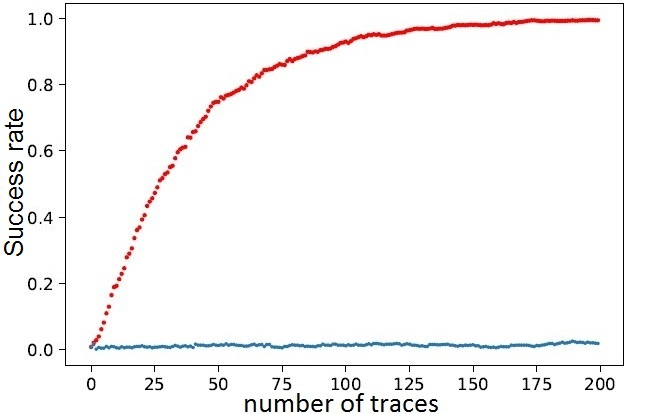
\includegraphics[scale=0.32]{Fig/200_D1.PNG}}    
    \subfigure[$D=2$]{\label{fig:200_D2}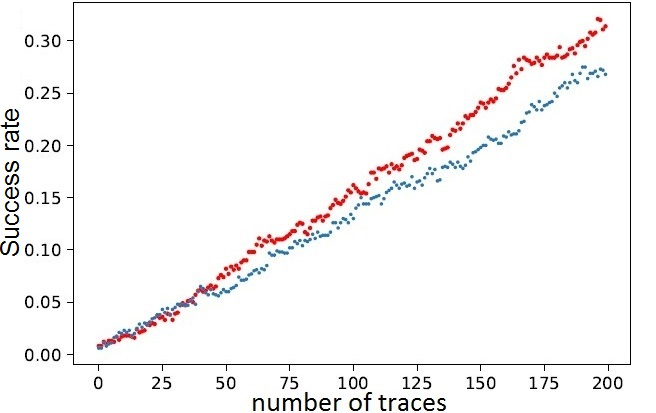
\includegraphics[scale=0.32]{Fig/200_D2.PNG}}
    \subfigure[$D=3$]{\label{fig:200_D3}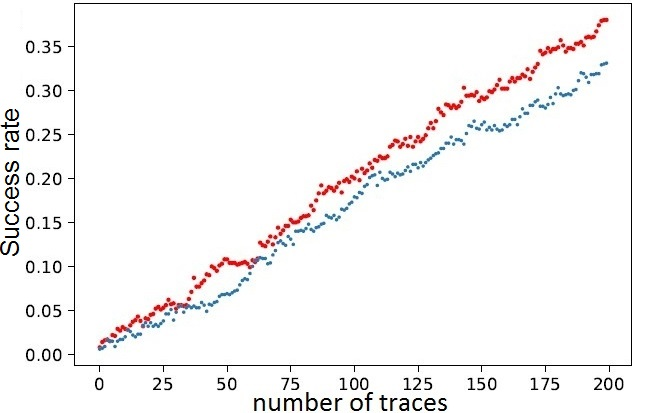
\includegraphics[scale=0.32]{Fig/200_D3.PNG}}
    
    \subfigure[$D=4$]{\label{fig:200_D4}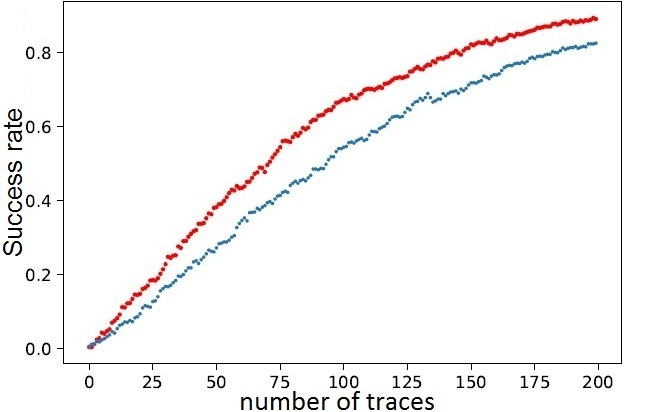
\includegraphics[scale=0.32]{Fig/200_D4.PNG}}
     \subfigure[$D=5$]{\label{fig:200_D5}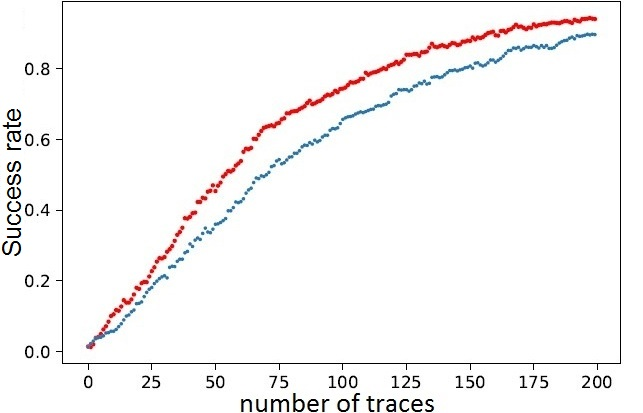
\includegraphics[scale=0.32]{Fig/200_D5.PNG}}    
    \subfigure[$D=10$]{\label{fig:200_D10}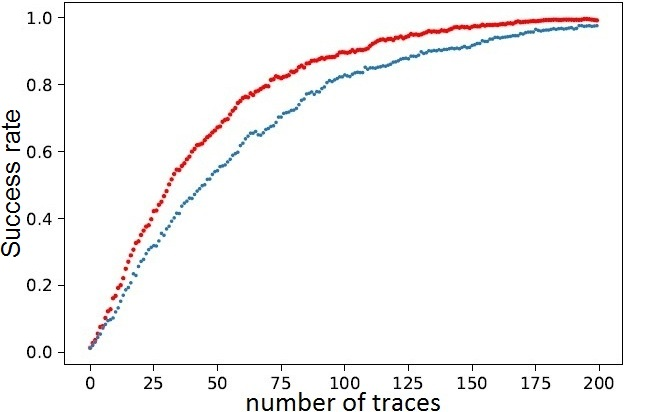
\includegraphics[scale=0.32]{Fig/200_D10.PNG}}
    
    \subfigure[$D=20$]{\label{fig:200_D20}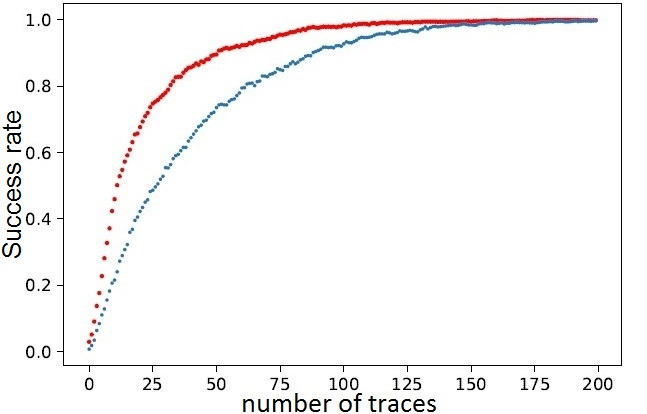
\includegraphics[scale=0.32]{Fig/200_D20.PNG}}    
    \subfigure[$D=30$]{\label{fig:200_D30}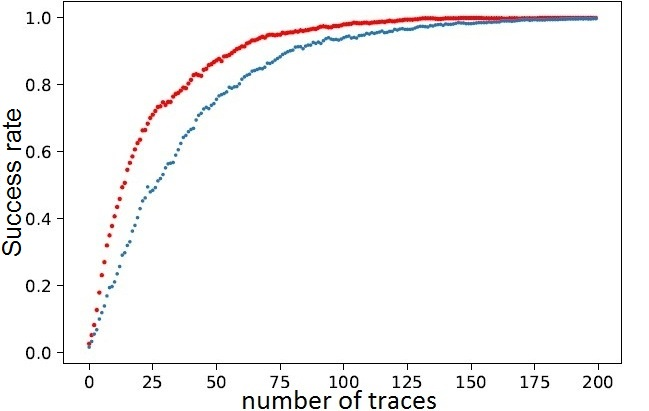
\includegraphics[scale=0.32]{Fig/200_D30.PNG}}
    \subfigure[$D=50$]{\label{fig:200_D50}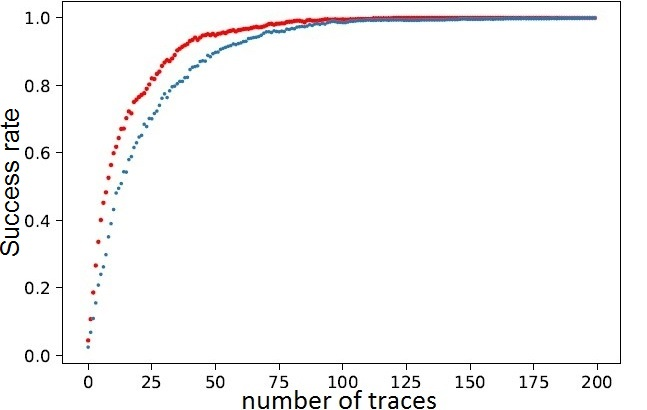
\includegraphics[scale=0.32]{Fig/200_D50.PNG}}
   
    \caption{Success rate according to the number of traces (\colorbox[rgb]{0.9,0.9,0.9} {until $N=200$}), for different values of $D$, with: ({\color{blue}{$\bullet$}}): coalescence and ({\color{red}{$\bullet$}}): our improvement}
    
    \label{fig:200}
\end{figure*}



  \begin{figure*}%[H]
    \centering
    \subfigure[$D=1$]{\label{fig:1000_D1}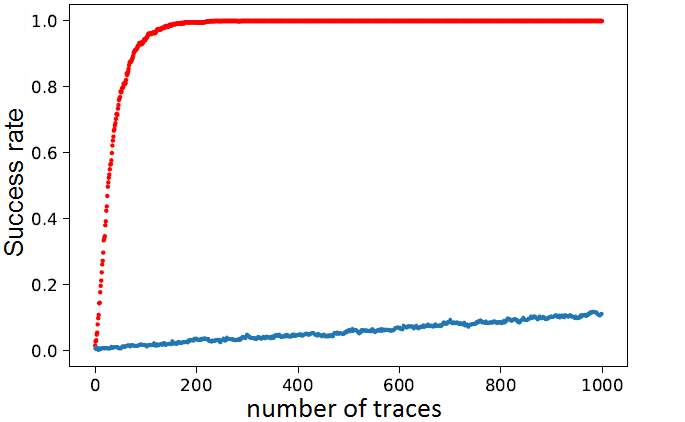
\includegraphics[scale=0.46]{Fig/1000_1.PNG}}
    \subfigure[$D=2$]{\label{fig:1000_D2}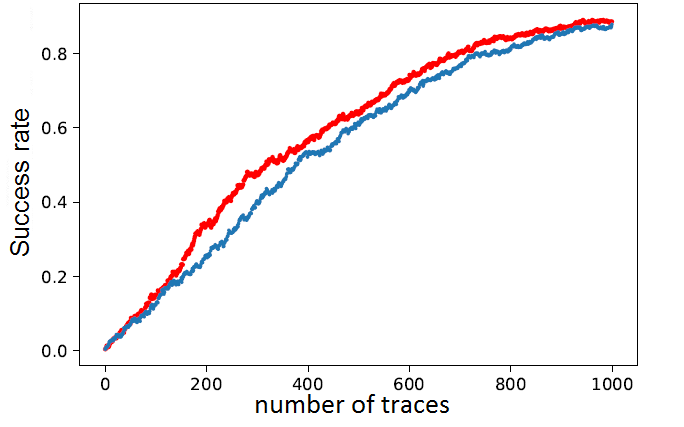
\includegraphics[scale=0.46]{Fig/1000_2.PNG}}
    %\subfigure[$D=3$]{\label{fig:1000_D3}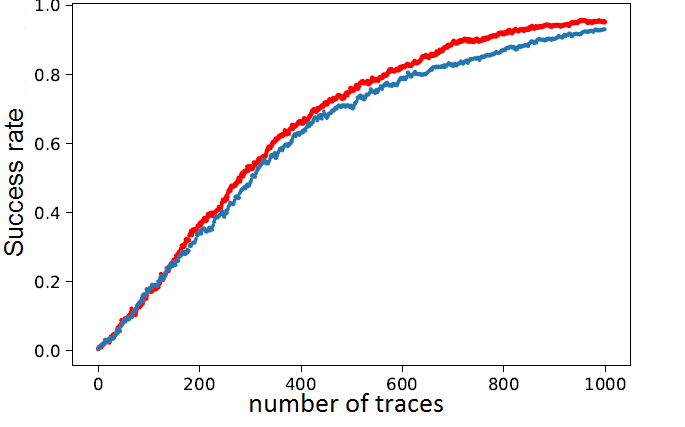
\includegraphics[scale=0.46]{Fig/1000_3.PNG}}
    %\subfigure[$D=4$]{\label{fig:1000_D4}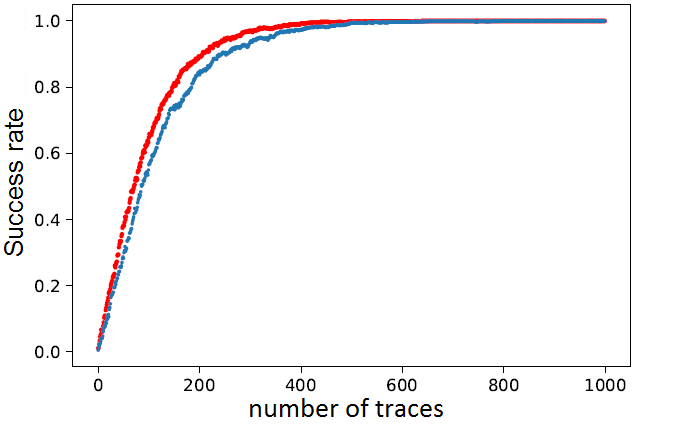
\includegraphics[scale=0.46]{Fig/1000_4.PNG}}
    \subfigure[$D=5$]{\label{fig:1000_D5}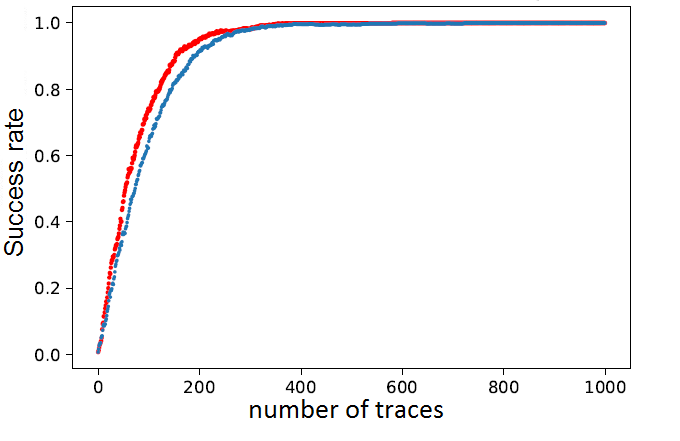
\includegraphics[scale=0.46]{Fig/1000_5.PNG}}
   
    \caption{Success rate according to the number of traces (\colorbox[rgb]{0.9,0.9,0.9} {until $N=1000$}), for different values of $D$, with: ({\color{blue}{$\bullet$}}): coalescence and ({\color{red}{$\bullet$}}): our improvement}
    \label{fig:1000}
\end{figure*}
  
%\vspace{1 cm}
%\todo[inline]{In Practice, For $D=1$ (monovariate attack), our approach is significantly better than the old one. This results from....For $D>1$, our approach is less significantly better than the old one (especially for a large number of messages). With a larger dimensionality (i.e., when $D$ grows), the success rate converges faster to 100\% for both approaches.}

In practice and interestingly, when $D=1$ (mono-sample attack), we notice that the success rate with coalescence requires a lot of traces to start differing from $0\%$.
On the other hand, with our exact computations, the success rate in the mono-sample case is increasing fast to $100\%$.
It is even faster than the case of exact computation when $D>1$.
This fact can be explained by the selection of the (unique) point of attack.
We selected the point where our attack succeeds the best (i.e., with the best signal-to-noise ratio).
So, adding more points comes down to adding (relatively) less information.
For clarity, we represented the value of the success rate (after an arbitrary number of $100$ matching traces) for attacks with coalescence and with our improvement (exact template computation) in figures~\ref{fig-sr_D1_SAMPLE100_coalescance} and~\ref{fig-sr_D1_SAMPLE100_exact}.
The sample of attack for the graphs in Fig.~\ref{fig:1000} corresponds to the best sample (at position $350$).
This sample has a very higher SNR compared to its neighboring samples, which makes it very singular.
This accounts for the fact the exact attack at $D=1$ exhibits a better success rate than for $D>1$ (until approximately $D=5$).
From $D=5$ on (i.e., large dimensionality), we recover the fact that the higher $D$, the higher the success rate (since there is no longer a big discrepancy between the added points, in terms of SNR). Noting that each trace contains $700$ samples. 

\begin{figure}
\begin{center}
\includegraphics[width=0.7\linewidth]%[width=0.93\linewidth]
{Fig/sr_D1_SAMPLE100_coalescance.png}
\end{center}
\caption{Success rate after 100 traces for $D=1$ in the (legacy) coalescence approach, as a function of the sample chosen for the attack.}
\label{fig-sr_D1_SAMPLE100_coalescance}
\end{figure}

\begin{figure}
\begin{center}
\includegraphics[width=0.66\linewidth]%[width=0.88\linewidth]
{Fig/sr_D1_SAMPLE100_exact.png}
\end{center}
\caption{Success rate after 100 traces for $D=1$ in our new exact approach, as a function of the sample chosen for the attack. It shows that the selection of the sample $350$ is definitely singular, as the attack is significantly better at this sample than at others, even its neighbors.}
\label{fig-sr_D1_SAMPLE100_exact}
\end{figure}

\begin{table*}%[htb]
		\caption{Computation time (seconds) according to the traces dimensionality $D$.} 
		\label{tab3}	
	\setlength{\extrarowheight} {2pt}
\large	
	\begin{center}
		\begin{tabular}{|c|c|c|c|c|c|c|c|c|c|}
			\cline{2-10}
			\multicolumn{1}{c|}{} & \bf 1   & \bf 2   & \bf 3   & \bf 4   & \bf 5   & \bf 10   & \bf 20   & \bf 30   & \bf 50 \\\hline
			\bf  
			
			\bf Coalescence 
			& 26.649 & 29.658 & 31.980 & 35.021 & 37.158 & 55.814 & 75.392 & 105.150 & 159.486  \\\hline
			\bf Improvement
			& 31.365 & 33.128 & 35.801 & 37.964 & 39.754 & 54.016 & 82.036 & 106.676 & 170.333 \\\hline
			
		\end{tabular}
	\end{center}
\end{table*}
  
 
%\twocolumn

In order to study and compare the computation time for the two approaches (coalescence and our improvement), we run them by varying the window $D$ from $1$ to $50$, while setting the number of traces to a given value ($200$ in our case). The execution times obtained are given in Table~\ref{tab3} and plotted in Figure~\ref{temps de calcul}.

\begin{figure}[H]
\begin{center}
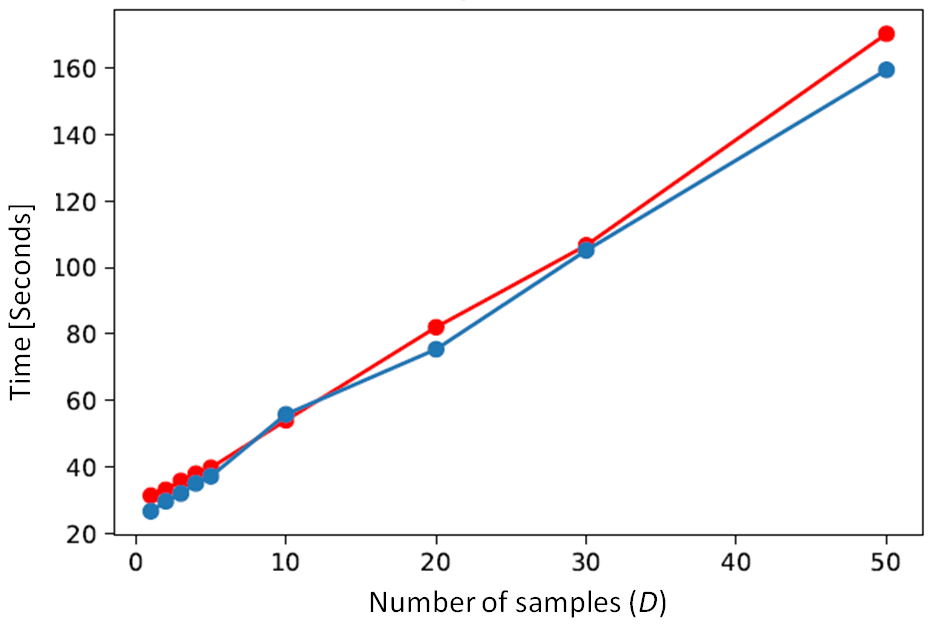
\includegraphics[width=1.0\linewidth]{Fig/temps_de_calcul.PNG}
\end{center}
\caption{Computation time according to $D$ with: ({\color{blue}{$\bullet$}}): coalescence and ({\color{red}{$\bullet$}}): our improvement}
\label{temps de calcul}
\end{figure}

%\todo[inline]{Est-ce possible dans la figure 3 de mettre D en italique dans la légende des $X$, et de mettre ``Time [seconds]'' dans la légende des $Y$ ?} % Done
 
From the above experimental results, we can see that our approach offers a considerable improvement in terms of success rate at the expense of a marginal delay in terms of computation time. 
This shows the importance of this improvement, as in general an improvement of say 10\% in data (number of traces complexity is much more valued than an improvement of 10\% in computational complexity).
   
%\section{Amélioration des attaques basées sur la régression linéaire LRA}


\section{Conclusion and perspectives}\label{sec-conclusion}

In this paper, we described a new improvement in template attacks' success rate and computational speed.
We took advantage of the properties of the spectral approach and were inspired by the coalescence principle, while mathematically demonstrating the optimality of the proposed improvement.

Furthermore, we presented a validation consisting of practical results obtained in the form of graphs, clearly showing the improvement in success rate compared with the previous version of coalescence-based template attacks. 
This considerable gain in success rate comes at the expense of a marginal loss in computation time, which is explained in terms of complexity.

Besides, the application of the coalescence principle was introduced in attacks based on linear regression (as early as the first LRA paper~\cite{DBLP:conf/pkc/Schindler05}). 
Recall that it causes accuracy errors, with template attacks, due to class imbalance.
So, it seems that our improvement of template attacks could be extended to the linear regression-based one, by taking into account the class sizes and getting inspiration from the spectral computation~\cite{DBLP:conf/cosade/OULADJ2020}. 
This work is planned as a future improvement, as thus left as a perspective.


\bibliographystyle{plain}
\bibliography{sca}

\end{document}
